%% This is an abbreviated template from http://www.sigplan.org/Resources/Author/.

\documentclass[acmsmall,review,authorversion]{acmart}
\acmDOI{}
\acmJournal{FACMP}
\acmVolume{CSCI 5535}
\acmNumber{Spring 2020}
\usepackage{graphicx}
\usepackage{amssymb}
\usepackage{mathtools}
\usepackage{amsmath}
\usepackage{subcaption}
\captionsetup[subfigure]{width=0.9\textwidth}
% If we want to distinguish captions and the main text more
% \captionsetup[figure]{width=0.9\textwidth}
% \captionsetup[table]{width=0.9\textwidth}
\usepackage[linesnumbered,ruled]{algorithm2e}
% \graphicspath{ {./assets/} }
\SetKwRepeat{Do}{do}{while}

\begin{document}

%%
%% The "title" command has an optional parameter,
%% allowing the author to define a "short title" to be used in page headers.
\title{A Framework for Formal Verification to Correct Actions in Reinforcement Learning}

%%
%% The "author" command and its associated commands are used to define
%% the authors and their affiliations.
%% Of note is the shared affiliation of the first two authors, and the
%% "authornote" and "authornotemark" commands
%% used to denote shared contribution to the research.
\author{Ethan Hobbs}
\email{ethan.hobbs@colorado.edu}
\author{Vikas Nataraja}
\email{viha4393@colorado.edu}
\affiliation{%
  \institution{University of Colorado Boulder}
}


%%
%% The abstract is a short summary of the work to be presented in the
%% article.

\begin{abstract}
In reinforcement learning, proving the possibility of a safe state is inherently difficult due to the range of methods available to find a new safe state. One of the most common approaches for finding a new state when the agent reaches an unsafe one is reverting to an initial state. In many cases, these methods are inefficient or might not actually produce a safe state transition. In this paper, we propose a new method for verifying an agent's policy for transitioning out of an unsafe state in the immediate future by using backtracking to guarantee safe state transition.
\end{abstract}

%%
%% This command processes the author and affiliation and title
%% information and builds the first part of the formatted document.
\maketitle

\section{Introduction}
\label{section:intro}
Reinforcement Learning (RL) has gained immense momentum in recent years particularly in the field of robotics where tasks are repetitive and RL can make an instant impact. This is because the agent can learn a policy that maximizes the reward function much quicker in repetitive tasks because the reward environment is denser and guarantees near-continuous rewards for every action that the agent takes. With RL gaining popularity, verification of such systems is an active area of research in Computer Science. The core problem of any software verification is to verify that a given system satisfies its specification. A conventional way to verify validity is to establish safety rules before the agent is deployed in the environment which requires extensive data and pre-computation \cite{gopinath:2017}. It is not always possible to predict the states or the changes in the environment beforehand particularly if it is dynamically changing. Another common approach that is more widely deployed in Machine Learning is for the system itself to verify its own progress \cite{zhu:2019,sun:2019}. While it is difficult to characterize such a verification, it affords better safety which is essential in RL (and relational verification of RL). Formal state verification then becomes essential so that the agent can monitor its progress by checking the validity of states. We propose \emph{backtracking} through past states to avoid transitioning to an invalid or unsafe state similar to the method proposed by Goyal et al. \cite{DBLP:journals/corr/abs-1804-00379}

In this paper, we address the problem of overcoming invalid or unsafe states by presenting an extension to \cite{zhu:2019}. First, we introduce a toy problem explaining our process, the terminology that will be used in the rest of the paper, describing and defining the basis functions followed by a technical section explaining the theoretical background behind our implementation. We then present an evaluation scenario and round out by discussing the conclusion and future work and improvements.

\section{Overview}
\label{section:overview}

    
    
In traditional reinforcement learning systems, an agent can get stuck in a situation where there are no safe actions that allow the system to progress. This is especially apparent in physical systems like a robotic arm where to get to a new state, the robot might cause damage to itself. An example situation can be seen in Figure \ref{fig:ex1} and \ref{fig:ex2}. Here the agent transitions from state 1 to 2 which is a valid action that is safe. However there are no actions at this location that are safe so the learning process would stop leaving the agent untrained.

    \begin{figure}[htb]
        \centering
        \begin{subfigure}{.5\textwidth}
          \centering
          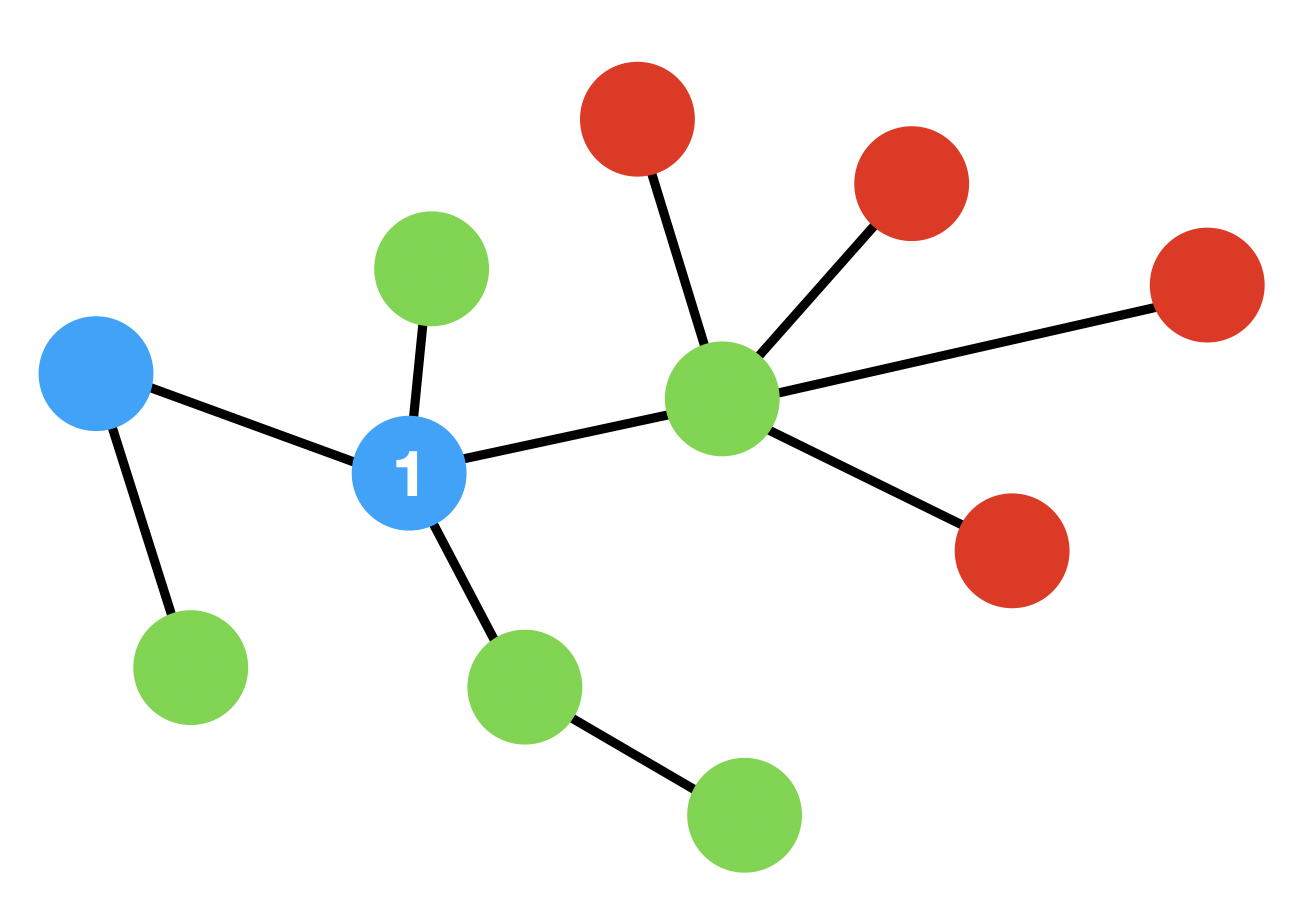
\includegraphics[width=.8\linewidth]{assets/example_1.png}
          \caption{Initial state labeled state 1}
          \label{fig:ex1}
        \end{subfigure}%
        \begin{subfigure}{.5\textwidth}
          \centering
          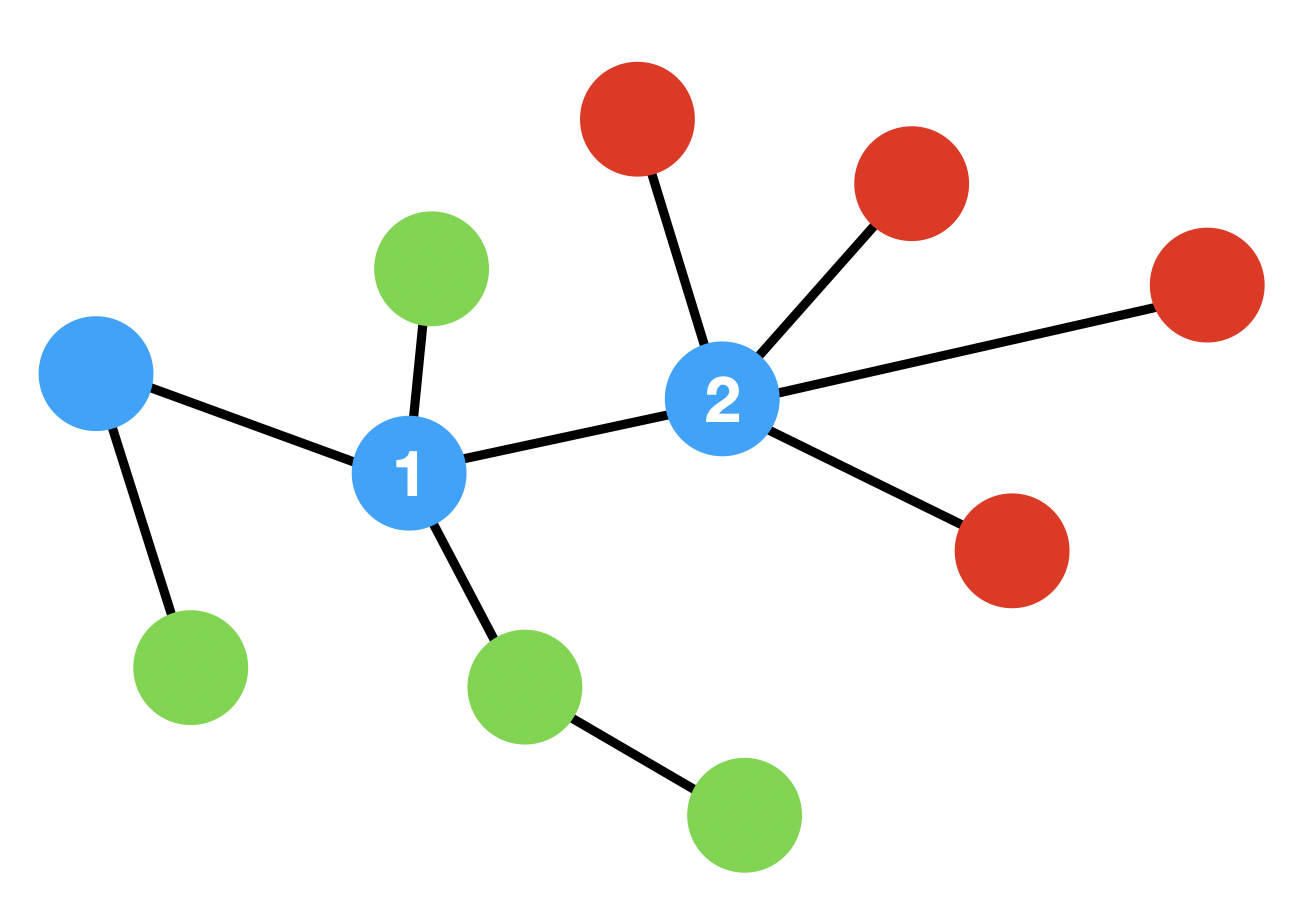
\includegraphics[width=.8\linewidth]{assets/example_2.png}
          \caption{New state at 2. Notice there are no safe states to transition to.}
          \label{fig:ex2}
        \end{subfigure}
        \begin{subfigure}{.5\textwidth}
          \centering
          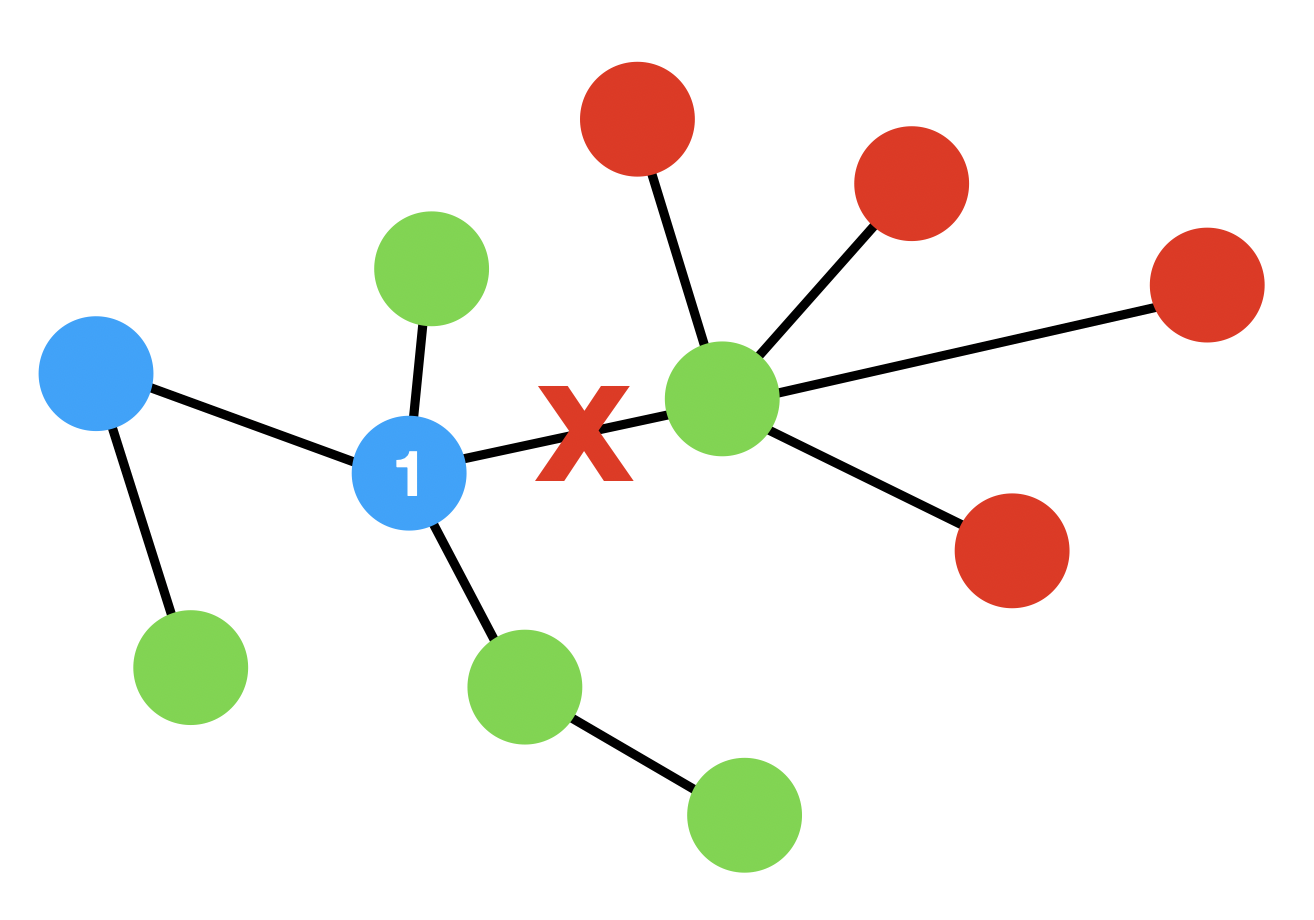
\includegraphics[width=.8\linewidth]{assets/example_3.png}
          \caption{Backtracking step to state 1 avoiding being stuck. The red x indicates that the transition to former state 2 is no longer possible}
          \label{fig:ex3}
        \end{subfigure}%
        \begin{subfigure}{.5\textwidth}
          \centering
          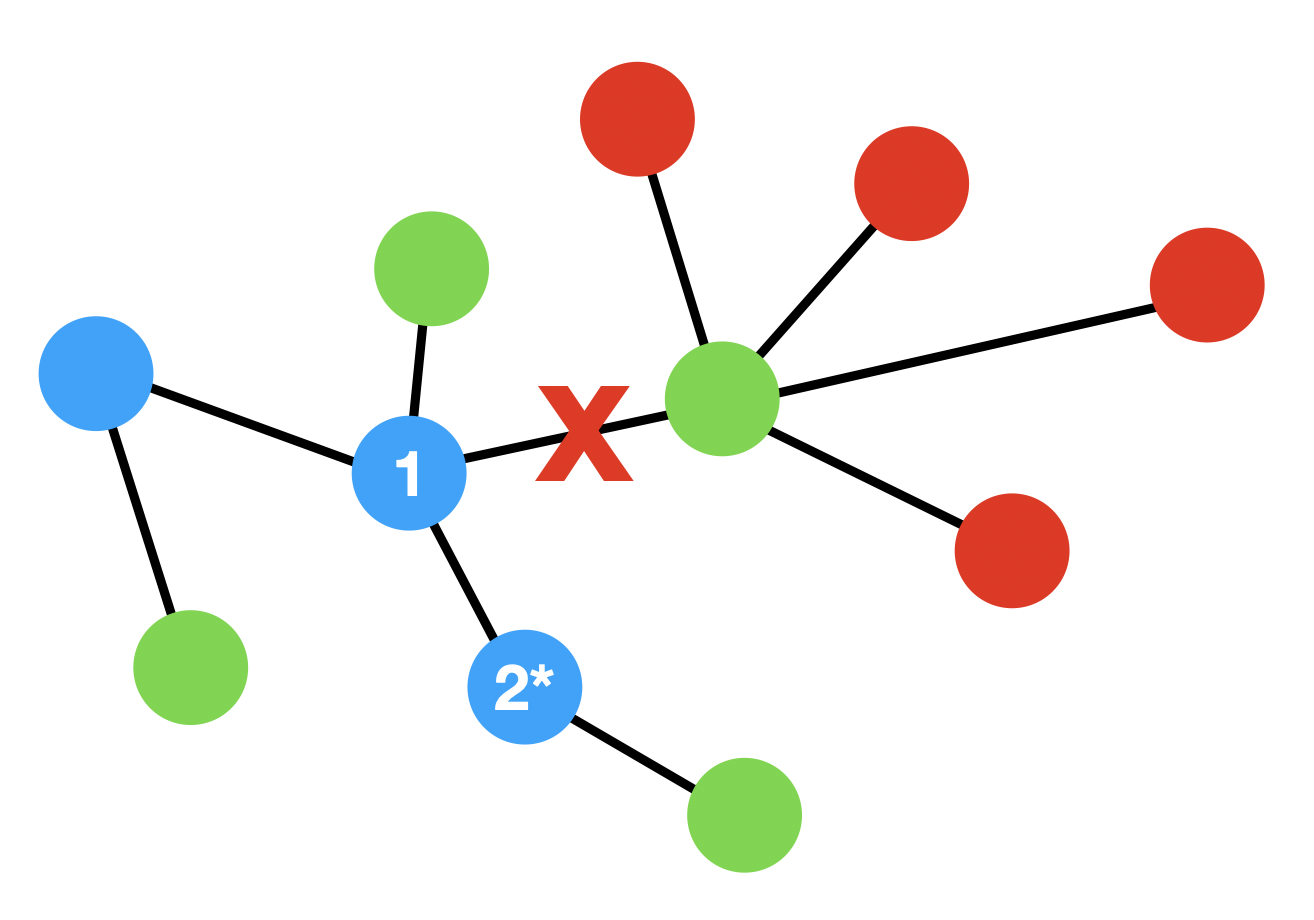
\includegraphics[width=.8\linewidth]{assets/example_4.png}
          \caption{Repeating the process at state 1 leads us to state $2^*$.}
          \label{fig:ex4}
        \end{subfigure}
        \captionsetup{justification=centering}
        \caption{A toy example of backtracking. The blue indicates states that exist in memory. The green indicate safe states while the red indicate unsafe states.}
        \label{fig:example_system}
    \end{figure}
    
To make the system more intuitive, we consider a cartpole system which is an extension of the classical inverted pendulum problem. A pole is attached by an un-actuated joint to a cart, which moves along a frictionless track. A visual reference can be seen in Figure \ref{fig:cartpole}. The system is controlled by applying a discrete force measure to the cart. The pendulum starts upright, and the goal is to prevent it from falling over. Assuming a \emph{fully observable} system, the observation space then becomes the cart velocity, cart position, pole angle and the pole velocity at the tip. Using these parameters, again, under the assumption that these are fully observable, we can describe the entire system. The action space is discrete and binary - moving the cart to the left or the right but not both. More details about the dynamics and specifics of the cartpole environment are explained in Section \ref{section:evaluation}. Using intuition, an unsafe state in this environment could potentially be if the proposed action caused damage to the cart such as large force to the cart causing it to leave the designated track. We will be using the example of the cartpole system throughout the paper to explain our methodology.

One method to get around this problem of overcoming unsafe states was developed by Zhu et al. \cite{zhu:2019}. In this method they synthesize a deterministic program from the policy and verify the action based on that approximation. If they encounter an invalid state they perform a mathematical operation on the state space reducing its size. This method works very well, however since most reinforcement learning systems are physical systems like robots, it would be preferable to apply a physical based operation to help the verification instead of an abstract mathematical operation.

If an agent had some knowledge of its previous states, then, when it encountered an unsafe one, it could revert to a previous state and try a different path. We call this idea \emph{backtracking}. There are two components to this idea: a look ahead phase, and then a possible backwards step if there are no safe states. These components can be seen in Figure \ref{fig:ex3} and \ref{fig:ex4}. In Figure \ref{fig:ex1}, the agent is stuck at state 2 after completing the look ahead stage, but it has a memory of the current and previous states shown in blue. We revert back to state 1 and eliminate the possibility of taking the same transition. The agent then makes a new choice of the possible states and enters into state $2^*$ thus avoiding the invalid states. 

    \begin{figure}[ht]
        \centering
        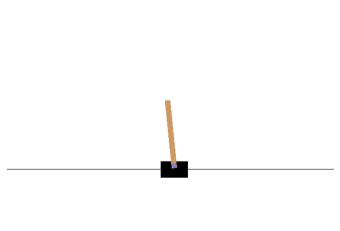
\includegraphics[width=0.5\textwidth]{assets/cartpole.png}
        \caption{Screenshot of the Cartpole-v1 environment}
        \label{fig:cartpole}
    \end{figure}

\section{Reinforcement Learning Background and Terminology}
\label{section:rl_background}
This section will detail some basic concepts in reinforcement learning such as Q-learning, policies, rewards and other common terminology used in reinforcement learning that will be used in subsequent sections.

    \begin{figure}[ht]
        \centering
        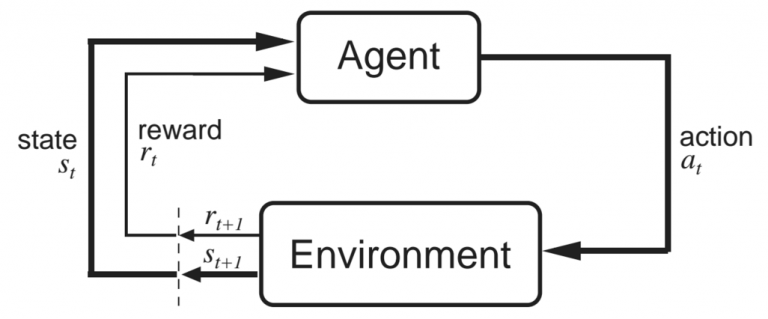
\includegraphics[width=0.65\textwidth]{assets/rl_schematic.png}
        \caption{Schematic representation of an RL agent and environment \cite{sutton1992reinforcement}.}
        \label{fig:agent_env}
    \end{figure}

\subsection{Q function, policy and reward}
\label{sub:qfunction}
In reinforcement learning, the objective is to maximize a certain \emph{reward} in a given situation. In our example of a cartpole, the objective is to balance the pole without having it fall over and for every timestep that is achieved, a positive reward is received. It is important to consider immediate rewards and future rewards simultaneously because optimizing for one means sacrificing the other and this concept of exploration vs exploitation is a core concept of RL and we use $\gamma$ to indicate the \emph{discount factor} which balances these two types of policies. To quantify reward, formally we can write the cumulative discounted reward as:

\begin{equation}
\label{eq:reward}
    R_t = \sum_{t=0}^{\infty} \gamma^k r_t
\end{equation}

\noindent where $t$ indicates timestep, \emph{$r_t$} is the expected reward at timestep $t$. \\

Next, we introduce \emph{policy} as describing the way of taking an action or more specifically, it describes the probability of taking an action in a given state. It takes in an action and a state and return the probability of taking that action with the goal being to maximize over some parameter(s) $\theta$. It is denoted by $\pi_{\theta}(s,a)$ or sometimes $\pi_{\theta}(a|s)$ as a way of indicating conditional probability. We will use the former notation in this text.

Using these terms, we can formalize an action value function called $Q$ which indicates the value of taking action $a$ in state $s$ when acting under a policy $\pi$ as the expectation of receiving reward $R_t$ when in state $s$ and taking action $a$:

\begin{equation}
\label{eq:q_function}
    Q^\pi (s, a) = \mathbb{E}_\pi [R_t|S_t = s, A_t = a]    
\end{equation}

The expectation takes into account the randomness in future actions according to the policy, as well as the randomness of the returned state from the environment. The randomness arises because both the policy and the transition function to go from one state to the other may be stochastic. Figure \ref{fig:agent_env} describes the schematic relationship between an agent and its environment. At a time step $t$, the agent is in state $s_t$ and takes an action $a_t$. The environment then responds with a new state $s_{t+1}$ and a reward $r_{t+1}$. The reason that the reward is at $t+1$ is because it is returned with the environment with the state at $t+1$. 

\subsection{Q-learning}
\label{sub:qlearning}
Q-learning was first introduced in 1992 by Watkins et al. as a way for an RL agent to learn an optimal policy in a Markov Decision Process (MDP) \cite{Watkins92q-learning}. Since then, it has gained immense popularity and is one of the most common ways of learning a policy. It uses the $Q$ function to learn a policy for a state-action pair. In this context, $Q$ function is the action value function that indicates the value of taking a particular in some state under a policy $\pi$. At the start of the episode or session, all Q values are either initialized with zeros or randomly initialized. For each state, every action possible at that state has an associated reward for taking that action and it should be noted that rewards can be negative as well to indicate that the agent chose the "wrong" action and learned a sub-optimal policy and these negative rewards are cumulatively used to learn a better policy at each timestep depending on the reward. After every action is taken and an outcome is observed, the $Q$ value is updated. At each timestep, the maximum expected future reward is balanced against optimizing current state-action policy by using $\gamma$. To update the $Q$ value from the previous $Q$ value we use the expected reward (of taking action $a$ at state $s$ ) and the maximum of the predicted $Q'$ value over a possible future state $s'$ and action $a'$ influenced by the discount factor $\gamma$. We also introduce \emph{learning rate} $\alpha$ which balances the extent to which the new $Q$ value is considered over the previous one. Putting this together, we arrive at this equation:


\[\underbrace{\text{New}Q^{\pi}(s,a)}_{\scriptstyle\text{New  Q-Value}}=Q^{\pi}(s,a)+\mkern-34mu\underset{\text{Learning Rate}}{\underset{\Bigl|}{\alpha}}\mkern-30mu[\underbrace{R(s,a)}_{\scriptstyle\text{Reward}}+\mkern-30mu\underset{\text{Discount factor}}{\underset{\Biggl|}{\gamma}}\mkern-75mu\overbrace{\max Q'(s',a')}^{\scriptstyle\substack{\text{Maximum predicted reward, given} \\ \text{new state and all possible actions}}}\mkern-45mu-Q(s,a)]\]


\subsection{Deep Q-learning}
\label{sub:deep_q}

Deep Q-learning is an extension of the Q-learning scheme and improves upon it by speeding up the learning process using deep neural networks and reduces memory consumption. Classical Q-learning works well for environments with a small number of states and actions because the Q-table can be easily built. But it cannot handle computation for environments having hundreds or thousands of states and actions because saving the Q-table in memory is simply unrealistic. Deep Q-learning overcomes this problem by approximating the Q-value using neural networks trained as a regression problem and evaluated under appropriate loss functions like mean squared error. For each state, it approximates the actions and chooses the \emph{best} action for that state and records progress in the experience replay buffer. In our proposed method, we employ a deep Q-network to solve the evaluation scenario, more details about the implementation are available in Section \ref{section:evaluation}.

    \begin{figure}[ht]
        \centering
        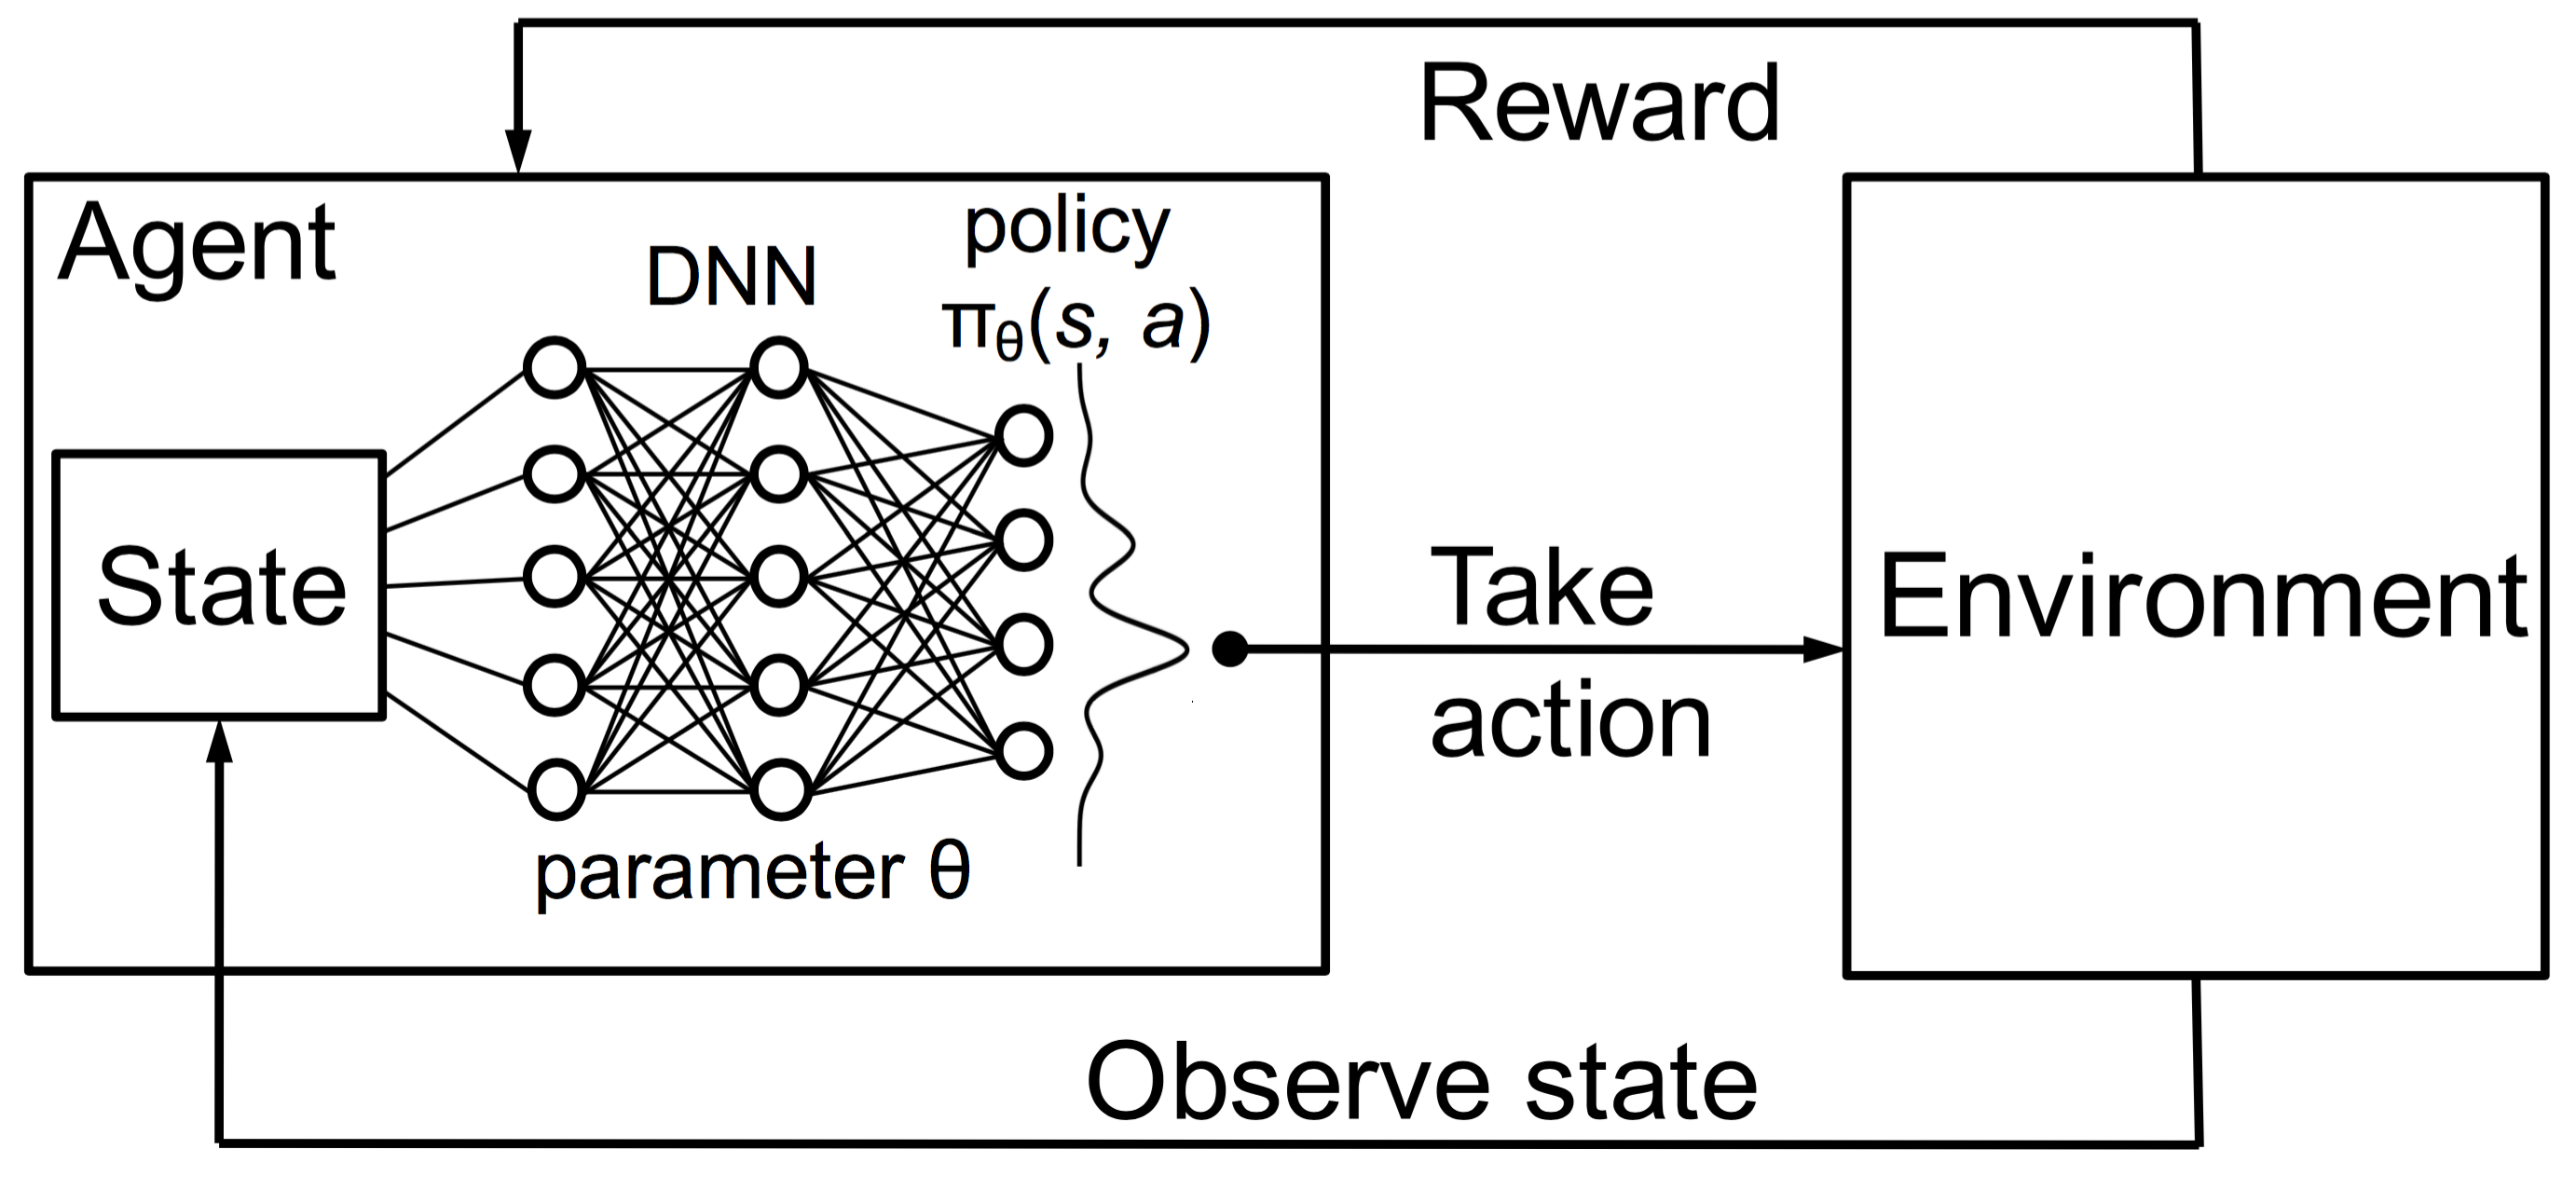
\includegraphics[width=0.65\textwidth]{assets/dqn.png}
        \caption{Schematic representation of a Deep Q-network \cite{10.1145/3005745.3005750}.}
        \label{fig:DQ_schem}
    \end{figure}

\subsection{Replay Buffer}
\label{sub:replay}
The replay buffer, also called experience replay, is a technique used to allow the agent to learn from previous experiences and thereby improving learning by making better informed decisions about the action to be taken at a state. The experiences are stored in a buffer with a preset memory size and the size of the memory can affect the speed of computation. Liu et al. explored the effects of changing memory sizes and found that too much or too little memory slow down the learning process \cite{DBLP:journals/corr/abs-1710-06574}. In our proposed work, we use the replay buffer to traverse through the history of saved states to find a safe state. The states in the buffer are guaranteed to be safe because the agent has continued learning and has updated its policies after passing those states.

\subsection{Unsafe or Invalid States}
\label{sub:unsafe_state}
Following the notation explained by Garcia and Fernandez \cite{DBLP:journals/corr/GarciaF14} we can define safe and unsafe states (also called error and non-error states) in RL as follows: \\

\emph{Let S be a set of states and $\phi \subset S$ the set of error states. A state $s \in \phi$ is an undesirable terminal state where the control of the agent ends when $s$ is reached with damage or injury to the agent, the learning system or any external entities. The set $\Gamma \subset S$ is considered a set of non-error terminal states with $\Gamma \cap \phi = \mathbb{\varnothing}$ and where the control of the agent ends normally without damage or injury.} \\

In the context of this paper, we describe an error state as an undesirable state that if entered, the episode ends abruptly and could cause harm to the program. Our aim with this paper is to show that when an unsafe state is encountered (or is about to be encountered), instead of reverting to a set of initial states, we can backtrack through the agent's recorded states and history in the replay buffer.

% \section{(Contribution 1)}

\section{Verification Process}
\label{section:verification}

    \begin{figure}[ht]
        \centering
        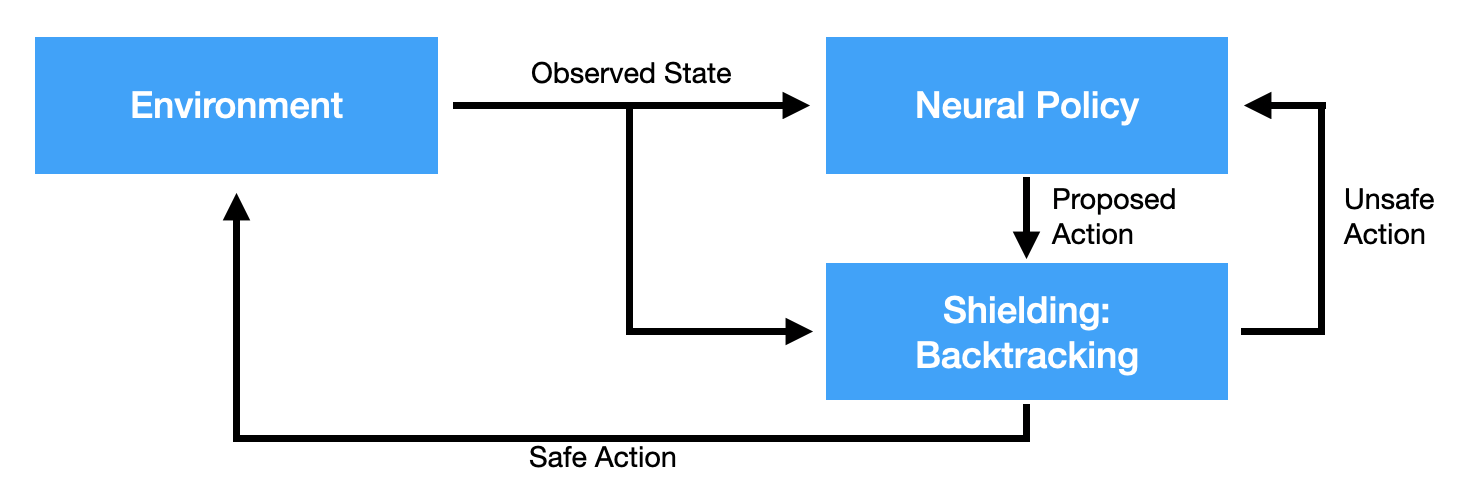
\includegraphics[width=0.65\textwidth]{assets/rl_flow_diagram.png}
        \caption{Modified flow of the reinforcement learning algorithm. Notice the inclusion of the sheilding step with two possible outputs: a safe action that updates the environment or an unsafe action which updates the neural policy.}
        \label{fig:sheilding_flow}
    \end{figure}
    
We chose to do a run time shielding method that will be assessed at each action taken by the agent. We follow the flow of the diagram in Figure \ref{fig:sheilding_flow} which is similar to the methods proposed in Zhu et al. \cite{zhu:2019}, but without the deterministic synthesis. We chose to do this since the more physical idea of backtracking was incredibly hard to abstract into the mathematical domain. There are several important factors to this verification step that can be tuned by the user as hyper parameters in the RL method: number of steps that the method looks ahead $n$, the number of states kept in the memory $m$, the number of steps previously that we start looking for a new state $thresh$ where $thresh \leq m$. 

Given the current state of the system $s$, and the developed policy $\pi$, we can begin the algorithm. First we must find all possible states $n$-steps ahead of the current state. We approach this by developing a tree with the number of leaves as the number of possible actions at each step. The set of each possible path of states is called $S_{possible}$. This method works for discrete systems with finite number of actions at each time step like the cartpole. We then must identify the safety of the states in $S_{possible}$ creating a new set of the safe states called $ S_{safe} \subseteq S_{possible}$. Identifying the safety of individual states is a hard problem on its own and outside of the scope of this paper. We chose an unrealistic method of manually inserting known invalid states while assuming all other states are safe states. Then we enter the shielding portion of the algorithm. If we have any possible states that are safe, we transition to them depending on the $Q$-function and add it to the replay buffer memory. Otherwise, we find a state $s_k$ in the replay buffer $R_b$ which we chose uniformly at random. We must then clear the replay buffer for every step after $s_k$ and repeat the algorithm until we have as safe action available to take. This method is summarized in Algorithm \ref{alg:verification}.


% We developed an algorithm (seen in Algorithm \ref{alg:verification}) that shows how this is possible. The first step is to synthesize a deterministic program with the method described in the previous subsection. With this deterministic approximation, we then can project forward in time $n$ number of steps in the future. In general we want this $n$ to be small for performance and speed purposes. This step allows us to see in the future what possible valid states there are as defined by the reinforcement learning scenario. If there is at least one valid state reachable from the current state in $n$ steps we proceed with the reinforcement learning and take the action determined by the policy. Otherwise if there are no valid states, we do not want to advance further down this path. Since we have discrete states, we chose to backtrack to the a previous safe state from $k$ steps ago and reclassify the current state as unsafe effectively cutting off the branch of the state network.

% In the verification, we look at a transition from state $a$ to state $b$ dependent on whether state $b$ is ``safe.'' Safe in this context means that the state is reachable by the reinforcement learning system and that it will not violate the failure conditions set out in the reinforcement system. 
    \begin{algorithm}[hbt]
    \
        Set threshold for backtracking timestep \emph{thresh} \\
        
        \Do{$S_{safe}$ is $\emptyset$}{
        $S_{possible}$ \leftarrow \text{Possible states from state $s$ $n$-steps ahead}\\
        
        $S_{safe}$ \leftarrow \text{Determine safe states in $S_{possible}$ dependent on $\gamma$} \\
        \eIf{$S_{safe}$ is not $\emptyset$}
          {
            $s' \in S_{safe}, \ a'$ \leftarrow \text{that maximizes New$Q^{\pi}(s',a')$}\\
            $R_b$ \leftarrow \ $R_b$ \cup \ \{s'\} \\
            % $Q^\pi (s, a) = \mathbb{E}_\pi [R_t|S_t = s, A_t = a]$ \\
            % New$Q^{\pi}(s,a) = Q^{\pi}(s,a) + \alpha [R(s,a) + \gamma.\max Q'(s',a') - Q(s,a)]$
          }
          {
            $\{s_k\} \in R_b$ \text{Chosen uniformly at random with} $k \geq thresh$ \\
            % Search replay buffer $R_b$ and choose random state with $k > thresh$ \\
            % $s = s_k$, $a = a_k$ \\
            remove all elements in $R_b$ before the updated $s_k$ and $a_k$\\
            Recalculate $Q^\pi (s_k, a_k)$ for the selected previous state
            %= \mathbb{E}_\pi [R_t|S_t = s, A_t = a]$ \\
            % New$Q^{\pi}(s,a) = Q^{\pi}(s,a) + \alpha [R(s,a) + \gamma.\max Q'(s',a') - Q(s,a)]$
            }
          }
          \Return state $s$, action $a$
     \caption{Shielding Algorithm (state $s$, policy $\pi$, replay buffer $R_b$)}
     \label{alg:verification}
    \end{algorithm}{}

\section{Empirical Evaluation}
\label{section:evaluation}
This section details our evaluation procedure and the experiment setup. We explain the inner workings of the dynamics of the chosen evaluation environment to tie it back to Algorithm \ref{alg:verification}.

Our proposed method was implemented in OpenAI Gym's cartpole environment \cite{DBLP:journals/corr/BrockmanCPSSTZ16}. Specifically, we implemented our model in the cartpole scenario, an extension of the inverted pendulum environment. The goal is to balance the cartpole without it falling over. The environment offers a discrete force unit of +1 and -1 using which the pole can be balanced. For every timestep that the pole doesn't fall over, a +1 reward is provided. Note that this can be changed to suit different positive discrete value. The state space, which is now fully observable because of dense rewards, becomes our observation space which can be seen in Table \ref{tab:cartpole}. The agent's episode ends when the pole is more than 15 degrees from vertical, or the cart moves more than 2.4 units from the center after which the environment resets and the subsequent episode starts. 

\begin{table}[hbt]
    \begin{tabular}{|l|l|l|l|}
    \hline
    Num & Observation & Min & Max  \\ \hline
    0 & Cart Position & -2.4 & 2.4 \\ \hline
    1   & Cart Velocity & $-\infty$ & $\infty$ \\ \hline
    2   & Pole Angle & $\sim -41.8^\circ$ & $\sim41.8^\circ$ \\ \hline
    3   & Pole Velocity at Tip & $-\infty$ & $\infty$ \\ \hline
    \end{tabular} 
    \caption{Observation Space constraints for Cartpole environment}
    \label{tab:cartpole}
\end{table}

To compare against, we chose the baseline to be a deep Q-network with 4 fully-connected or dense layers, each with non-linear ReLU (Rectified Linear Action Unit) activation except for the final layer which uses a linear activation because the output is a discrete value to be regressed over (the output of the network is an approximation of the action space which is discrete in our evaluation environment). Our proposed model implements a deep Q-network with state backtracking (not to be confused with neural network back propagation which uses gradients and derivatives to learn). Both models were trained with mean squared error loss function to learn the control policy of the environment. In the proposed model, we leverage the agent's state history which is already cached in the replay buffer (also called experience replay and memory replay). This also enables the agent to learn from off-policy experiences to better judge future state-action pairs. 

To get a fair comparison, we decided to record the scores for a total of 4 cases: baseline model evaluated under all valid states, proposed model evaluated under all valid states, baseline model evaluated under one random invalid state, and the proposed model evaluated under one random invalid state. We compared the scores in all 4 cases and fixed a threshold of 190 as recommended by OpenAI to mean "scenario solved" meaning when the model crosses a score of 190, it is considered solved. Additionally, we also fixed a pseudo-threshold of 2 for the number of times the model achieves a score of 190 meaning we consider the scenario to be solved when the model crosses 190 twice.
  
    \begin{figure}[thb]
        \centering
        \begin{subfigure}{.5\textwidth}
          \centering
          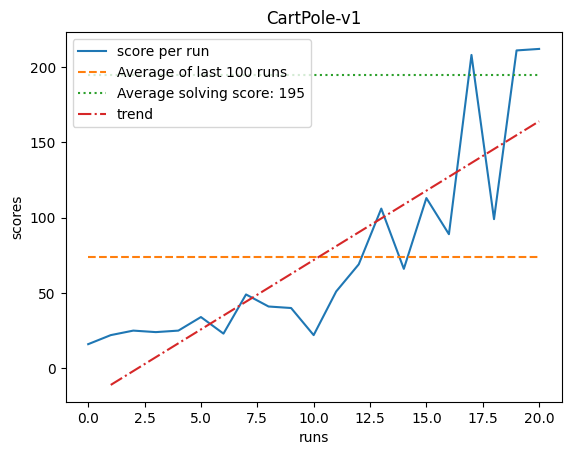
\includegraphics[width=.8\linewidth]{assets/baseline_valid.png}
          \caption{Baseline model evaluated with all valid states}
          \label{fig:baseline_valid}
        \end{subfigure}%
        \begin{subfigure}{.5\textwidth}
          \centering
          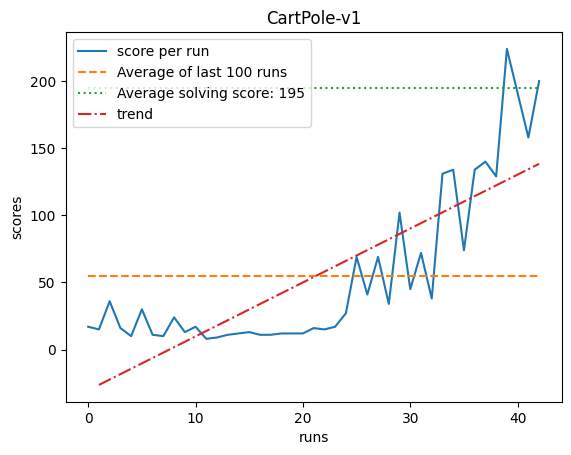
\includegraphics[width=.8\linewidth]{assets/backtrack_valid.png}
          \caption{Proposed model evaluated with all valid states}
          \label{fig:proposed_valid}
        \end{subfigure}
        \captionsetup{justification=centering}
        \caption{Baseline and proposed models evaluated under all valid states. Blue line shows the score per run/episode, orange line shows the average score of the past runs, green line shows the threshold of 190, red line tracks the trend of the scores}
        \label{fig:valid_states}
    \end{figure}
    
We observed that our model required more time to solve the cartpole environment when compared with a model that doesn't incorporate our changes in the absence of an invalid state. This is due to a combination of stochasticity of the environment and the fact that our look-ahead factor (the number of timesteps in the future to monitor for an invalid state) was quite large and thus resulted in computational speed. However, the total score achieved and the total reward remain largely the same. Figure \ref{fig:valid_states} shows the comparison between the two models' performances. It tracks the episodes or runs on the X-axis and the recorded score for that run on the Y-axis. The baseline model takes about 19 episodes to cross the 190 threshold for the second time while our proposed model takes 42 episodes. 
    
To test the model's performance in the presence of an invalid state, we forced one random element (with the same seed for both the baseline and the proposed models) of the observation space to go into an invalid form by replacing that element with a non-numerical state. Under these conditions, we noticed that the standard baseline model stopped as soon as it hit that state whenever that may be (due to the inherent stochasticity in the environment). Our model was able to detect the presence of the invalid state before entering it ahead of time and backtracked $k$ timesteps through its previous states to find an alternative albeit a temporarily sub-optimal policy. This resulted in the model overcoming the invalid state and thus finding a secondary derived policy which ultimately solved the scenario. Figure \ref{fig:invalid_state} shows the comparison between the two models. The baseline model stops after 5 episodes which is when it encounters the invalid state. The proposed model's score at episode 5 noticeably goes down for 3 episodes which is when it is computing an alternative policy. After episode 8, it recovers and the score starts increasing again and the model ultimately solves the scenario by crossing the 195 threshold for the second time at episode 26.

    \begin{figure}[hbt]
        \centering
        \begin{subfigure}{.5\textwidth}
          \centering
          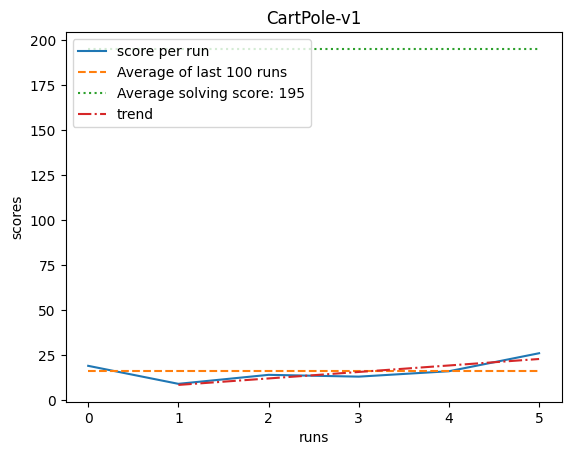
\includegraphics[width=.8\linewidth]{assets/baseline_invalid.png}
          \caption{Baseline model evaluated with one invalid state}
          \label{fig:baseline_invalid}
        \end{subfigure}%
        \begin{subfigure}{.5\textwidth}
          \centering
          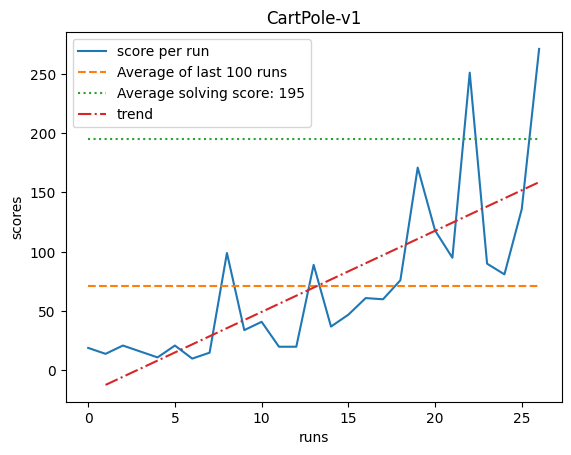
\includegraphics[width=.8\linewidth]{assets/backtrack_invalid.png}
          \caption{Proposed model evaluated with one invalid state}
          \label{fig:proposed_invalid}
        \end{subfigure}
        \captionsetup{justification=centering}
        \caption{Baseline and proposed models evaluated under one random invalid state.}
        \label{fig:invalid_state}
    \end{figure}


\section{Related Work}
\label{section:related_work}

In recent years, significant work has gone into verification of reinforcement learning and more specifically, the verification of states. A two-pronged system was implemented by Zhu et al. where the concept of safety and safety verification were both baked into the synthesis of a deterministic program with an inductive invariant alongside the neural policy \cite{zhu:2019}. However, when an invalid or incorrect state is observed, the agent reverts to one of initial safe states. In our approach, the agent back propagates to an already traversed safe state.
A similar formal verification approach was taken by Sun et al.  but to verify the actions of an autonomous robot by constructing a finite state abstraction and performing reachability analysis over the search space \cite{sun:2019}. However, if the initial set of safe states are not within a certain limit, there is a high risk of state space explosion. At the same time, it does not apply to unbounded states and does not capture the relationships between the state variables. These shortcomings are bypassed in our approach because we use the existing state space to find a safe state. Singh et al. introduced a method to certify deep neural networks by using a novel abstract interpreter which relies on a combination of floating-point polyhedra and activation functions such as ReLU (Rectified Linear Unit) and the sigmoid function \cite{singh:2019}. While this approach works to prevent exploding gradients during training, it works by transforming activation functions which inherently means that the neural network, in its current form, cannot be made robust to deeper architectures. In our proposed framework, we eliminate the need for changing activation functions by solving for state space. Chen et al. focused on relational verification represented as a Markov Decision Process (MDP) solvable via reinforcement learning \cite{chen:2019}. The problem with MDPs is that high-dimensional state spaces are not solvable. In our proposed method, we aim to use the existing policy to find a safe state which does not expand the dimensionality.



\section{Conclusion}
\label{section:conclusion}

We present an improvement to existing work to overcome unsafe or invalid states in reinforcement learning with the use of backtracking. Our proposed method requires more episodes to solve a scenario when there are no invalid states compared to baselines but performs comparably better when an invalid state is present in the observation space. Further, while the baseline fails to solve for invalid states, our model solves the scenario by opting for a sub-optimal policy for a temporary period and recovering to finish the scenario.


\section{Future Work}
\label{section:future_work}

Although our model performed well in the presence of an invalid state, we would like to experiment with multiple invalid states to test the robustness and adaptability of the model. One way to do this would be introduce additional invalid states at different stages which would allow us to evaluate the model's capability in such scenarios. One obvious shortcoming of our proposed model is the increased computational intensity. While this depends on the look-ahead factor i.e the number of states to look for in the future, we would like to make our model's performance time faster. One approach to do this would be to shorten the look-ahead factor so as to explore and search for fewer timesteps in the future but we would like to explore some other alternatives such as changing the model architecture as well. To test the model's versatility, we would like to explore other evaluation scenarios where learning a control policy is more nuanced and the environment has bigger observation and action spaces. 

\section{Online Resources}
\label{section:online_resources}
All our code and implementation can be found on our Github repository at this URL: \\ 
\url{https://github.com/csci5535-s20/project-rl-verification}.


\begin{acks}
We would like to thank Bor-Yuh Evan Chang and Benno Stein for their mentorship and advice during the course of this project.
\end{acks}

%%
%% The next two lines define the bibliography style to be used, and
%% the bibliography file.
\bibliographystyle{ACM-Reference-Format}
\bibliography{references}
\end{document}



% \begin{algorithm}[ht]
%     synthesize the deterministic program\\
%     Project forward $n$-steps\\
%     Check the validity of possible states \\
%     \eIf{valid states $\geq 1$}
%       {
%         proceed with reinforcement learning
%       }
%       {
%         return to the state $m$ states ago
%       }
%  \caption{Verification Algorithm}
%  \label{Alg:verif}
% \end{algorithm}{}

% \begin{algorithm}[hbt]
%     Synthesize the deterministic program \\
%     Project forward $n$-steps \\
%     Set threshold for backtracking timestep \emph{thresh} \\
%     Check the validity of possible future states dependent on $\gamma$ \\
%     \eIf{valid states $\geq 1$}
%       {
%         $Q^\pi (s, a) = \mathbb{E}_\pi [R_t|S_t = s, A_t = a]$ \\
%         New$Q^{\pi}(s,a) = Q^{\pi}(s,a) + \alpha [R(s,a) + \gamma.\max Q'(s',a') - Q(s,a)]$
%       }
%       {
%         search replay buffer history and choose random state with $k > thresh$ \\
%         $s = s_k$, $a = a_k$ \\
%         $Q^\pi (s, a) = \mathbb{E}_\pi [R_t|S_t = s, A_t = a]$ \\
%         New$Q^{\pi}(s,a) = Q^{\pi}(s,a) + \alpha [R(s,a) + \gamma.\max Q'(s',a') - Q(s,a)]$
%       }
%  \caption{Verification Algorithm}
%  \label{alg:verification}
% \end{algorithm}{}